% Bab 2  Tinjauan Pustaka
\chapter{TINJAUAN PUSTAKA}

\section{Studi Literatur}
Bagian ini memuat ulasan penelitian di bidang sejenis yang telah dilakukan oleh peneliti lain sebelumnya. Anda dapat mencantumkan hal-hal yang telah penulis pelajari dari literatur lain selama melakukan penelitian. Studi literatur sebaiknya menunjukkan pendekatan yang dilakukan oleh peneliti-peneliti sebelumnya dalam menjawab permasalahan penelitian. Semua sumber literatur yang digunakan di dalam subbab ini harus dicantumkan. Sitasi di dalam teks menggunakan gaya APA (\textit{American Psychological Association}) edisi ke-7 dengan format penulis--tahun, misalnya Andrews (2007) menyatakan bahwa ..., atau ... (Capozzi et al., 2013). Gunakan \textit{et al.} untuk sumber dengan tiga penulis atau lebih, dan tanda \& di dalam tanda kurung untuk dua penulis, misalnya (Xu \& Fischione, 2012).

\textit{Contoh kalimat bersitasi:} AlQahtani dan Alhassany (2013) membandingkan beberapa skema penjadwalan pada jaringan LTE. Penelitian tersebut sejalan dengan survei yang disusun oleh Capozzi et al. (2013). Kedua penelitian ini menjadi rujukan utama penelitian ini (AlQahtani \& Alhassany, 2013; Capozzi et al., 2013). Perbedaan dengan penelitian ini terletak pada …

\section{Tinjauan Teori}
Bagian ini memuat teori-teori yang berhubungan dengan penelitian. Pada bagian ini juga termuat dasar teori mengenai aplikasi dasar komponen atau piranti yang digunakan dalam sistem. Teori yang dimasukkan hanyalah teori-teori yang mendukung penelitian, misalnya konsep dasar analisis kestabilan di sistem kendali atau konsep dasar sistem komunikasi 4G. Teori dituliskan secukupnya sesuai kebutuhan. Jika terlalu panjang, teori-teori dapat diarahkan ke daftar pustaka yang digunakan.

\subsection{Sub Tinjauan Teori}
Penulis dapat membagi teori yang berhubungan dengan riset Penulis menjadi beberapa bagian. Tinjauan teori dapat menyertakan gambar dan tabel yang berfungsi sebagai penjelas dari teori yang Penulis sertakan. Selanjutnya akan diberikan penjelasan mengenai pembuatan dan penamaan tabel dan gambar yang disertakan di dalam laporan.

\textit{Contoh kalimat bersitasi:} Teori dasar sistem LTE dibahas secara menyeluruh oleh Ghosh et al. (2010). Rujukan pada halaman tertentu ditulis (Ghosh et al., 2010, hlm. 15). Kutipan langsung kurang dari 40 kata ditulis dalam tanda kutip dengan nomor halaman, misalnya menurut Andrews (2007, hlm. 3), “…kutipan langsung…”. Sumber yang dikutip dari sumber lain ditulis (Andrews, 2007, dalam Capozzi et al., 2013). Satu pernyataan yang didukung beberapa sumber dipisahkan dengan titik koma (Andrews, 2007; Xu \& Fischione, 2012).

\begin{singlespace}
\begin{longtable}{|c|p{0.38\linewidth}|p{0.44\linewidth}|}
\caption{Nama tabel}\\
\hline
\textbf{No} & \textbf{Nama Komponen} & \textbf{Fungsi} \\
\hline
1 & Komponen 1 & Penjelasan 1 \\
\hline
2 & Komponen 2 & Penjelasan 2 \\
\hline
3 & Komponen 3 & Penjelasan 3 \\
\hline
\end{longtable}
\end{singlespace}

Tabel 2.1 adalah contoh \textit{template} tabel yang dapat digunakan. Tabel harus dituliskan dengan menggunakan perintah masukan tabel yang tersedia di dalam Microsoft Word, bukan di-\textit{crop} melalui sumber lain. \textit{Text} di dalam tabel harus berspasi \textit{single} dengan jarak \textit{before} dan \textit{after} bernilai 0. Gunakan \textit{Caption} dan \textit{Cross Reference} untuk penamaan tabel. Tabel yang disertakan tidak boleh terpotong oleh batas halaman. Jika tabel yang digunakan membutuhkan lebih dari satu halaman, gunakan \textit{repeat header} tabel agar informasi tabel tidak terputus.

\begin{figure}[H]
\centering
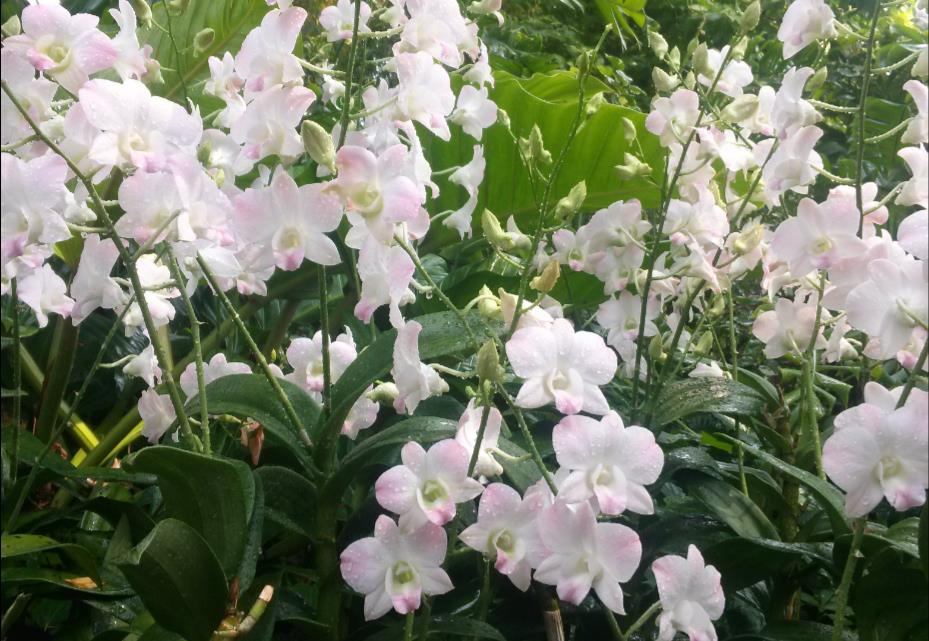
\includegraphics[width=0.5\textwidth]{../gambar/contoh-anggrek.png}
\caption{\textit{Dendrobium Peach}}
\end{figure}

Gambar 2.1 menunjukkan contoh \textit{template} untuk semua gambar yang digunakan di dalam laporan penelitian. Pastikan gambar yang disertakan memiliki resolusi yang mencukupi sehingga gambar dapat dilihat dengan jelas. Gambar adalah hasil gambar (foto) Penulis sendiri. Jika Penulis mengambil gambar dari sumber lain, pastikan untuk menyertakan sitasi (sumber gambar yang diambil). Selalu gunakan \textit{Caption} dan \textit{Cross Reference} dalam memberi nama dan mengacu gambar di dalam \textit{text}.

Gambar 2.2 menunjukkan contoh gambar grafik hasil penelitian. Gambar grafik dapat dibuat berwarna. Gunakan warna yang kontras untuk grafik berwarna yang disertakan. Warna yang kontras akan membuat grafik terlihat jelas saat dicetak berwarna. Ubah warna kontras menjadi garis hitam putih dengan pola titik-titik yang berbeda untuk \textit{hardcopy} hitam-putih. Gambar 2.3 menunjukkan contoh gambar grafik dengan warna hitam-putih. Penomoran gambar dan tabel menggunakan angka Arab, mengikuti urutan bab dan letak gambar/tabel di bab tersebut. Contoh: Gambar 2.2 artinya adalah gambar kedua yang ada di Bab 2, sedangkan Tabel 3.1 artinya adalah tabel pertama yang ada di Bab 3.

\begin{figure}[H]
\centering
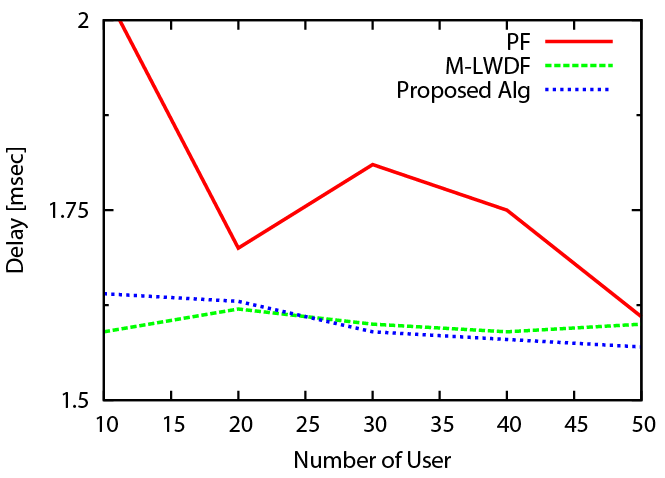
\includegraphics[width=0.55\textwidth]{../gambar/contoh-grafik-warna.png}
\caption{Hasil \textit{delay} warna terhadap penambahan pengguna}
\end{figure}

\begin{figure}[H]
\centering
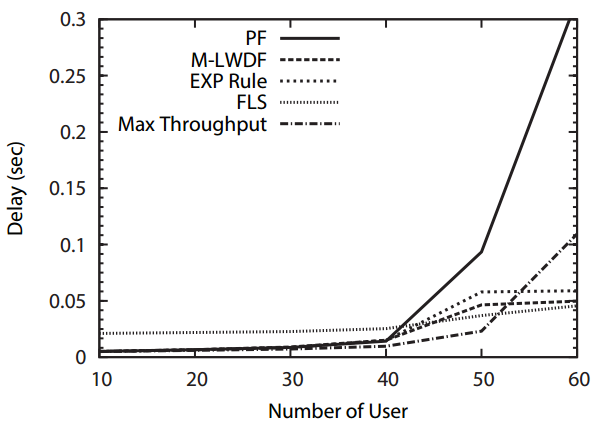
\includegraphics[width=0.55\textwidth]{../gambar/contoh-grafik-monokrom.png}
\caption{Hasil \textit{delay} monokrom terhadap penambahan pengguna}
\end{figure}

\subsection{Sub Tinjauan Teori 2}
\textit{Contoh kalimat bersitasi:} Sumber buku terjemahan ditulis dengan nama penulis aslinya (Gaman \& Sherrington, 1994), artikel berbahasa Indonesia (Radiati, 2000), dan sumber tanpa penulis memakai judul (\textit{Panduan penulisan karya ilmiah}, 2020).

Selalu gunakan perintah masukan persamaan yang disediakan oleh Microsoft Word. Jangan menggunakan potongan (\textit{crop}) persamaan dari literatur lain. Pastikan persamaan yang digunakan tertulis dengan jelas. Contoh \textit{template} persamaan ditunjukkan oleh Persamaan (2.1). Gunakan \textit{Caption} dan \textit{Cross Reference} untuk memudahkan pelacakan dan kompilasi semua persamaan yang digunakan di dalam dokumen. Nomor persamaan harus diletakkan di sisi kanan persamaan. Penggunaan tabel dalam contoh \textit{template} persamaan dimaksudkan untuk memudahkan penulisan \textit{caption} pada sisi kanan persamaan.

\begin{tanpagaris}
\begin{longtable}{@{}p{0.08\linewidth}>{\centering\arraybackslash}p{0.76\linewidth}r@{}}
 & $ds=\sqrt{r^{2}+\left(\dfrac{dr}{d\theta}\right)^{2}}\,d\theta$ & (2.1) \\
\end{longtable}
\end{tanpagaris}

dengan nilai:

\begin{tanpagaris}
\begin{longtable}{@{}p{0.15\linewidth}p{0.05\linewidth}p{0.6\linewidth}@{}}
$ds$ & = & penjelasan 1 \\
$dr$ & = & penjelasan 2 \\
$d\theta$ & = & penjelasan 3 \\
\end{longtable}
\end{tanpagaris}
